\documentclass{sigchi-ext}
% Please be sure that you have the dependencies (i.e., additional
% LaTeX packages) to compile this example.
\usepackage[T1]{fontenc}
\usepackage{textcomp}
\usepackage[scaled=.92]{helvet} % for proper fonts
\usepackage{graphicx} % for EPS use the graphics package instead
\usepackage{balance}  % for useful for balancing the last columns
\usepackage{booktabs} % for pretty table rules
\usepackage{ccicons}  % for Creative Commons citation icons
\usepackage{ragged2e} % for tighter hyphenation

% Some optional stuff you might like/need.
% \usepackage{marginnote}
% \usepackage[shortlabels]{enumitem}
% \usepackage{paralist}
% \usepackage[utf8]{inputenc} % for a UTF8 editor only

%% OVERRIDE THE DEFAULT COPYRIGHT STRIP
\copyrightinfo{Permission to make digital or hard copies of part or all of this work for personal or classroom use is granted without fee provided that copies are not made or distributed for profit or commercial advantage and that copies bear this notice and the full citation on the first page. Copyrights for third-party components of this work must be honored. For all other uses, contact the Owner/Author.\\
Copyright is held by the owner/author(s).\\
{\emph{TEI'17}}, March 20-23, 2017, Yokohama, Japan.\\
ACM XXX-X-XXXX-XXXX-X/XX/XX\\
\url{http://dx.doi.org/XX.XXXX/XXXXXXX.XXXXXXX}}

% Paper metadata (use plain text, for PDF inclusion and later
% re-using, if desired).  Use \emtpyauthor when submitting for review
% so you remain anonymous.
\def\plaintitle{Robot Skin: A Cloth Interface for Expressive Music Control}
  \def\plainauthor{First Author, Second Author, Third Author}
\def\emptyauthor{}
\def\plainkeywords{Authors' choice; of terms; separated; by
  semicolons; include commas, within terms only; required.}
\def\plaingeneralterms{Documentation, Standardization}

\title{Robot Skin: A Cloth Interface for Expressive Music Control}

\numberofauthors{3}
% Notice how author names are alternately typesetted to appear ordered
% in 2-column format; i.e., the first 4 autors on the first column and
% the other 4 auhors on the second column. Actually, it's up to you to
% strictly adhere to this author notation.
\author{%
    \alignauthor{%
        \textbf{Author1}\\
        \textbf{Author2}\\
        \affaddr{Institution} \\
        \affaddr{Country} \\
        \email{firstname@institution.org} }
    \alignauthor{%
        \textbf{Author3}\\
        \affaddr{Institution} \\
        \affaddr{Country} \\
        \email{firstname.lastname@gmail.com} \\
        \email{~} \\
        \email{~} }
    % use this blank space to show an overview of the project
    \mbox{ 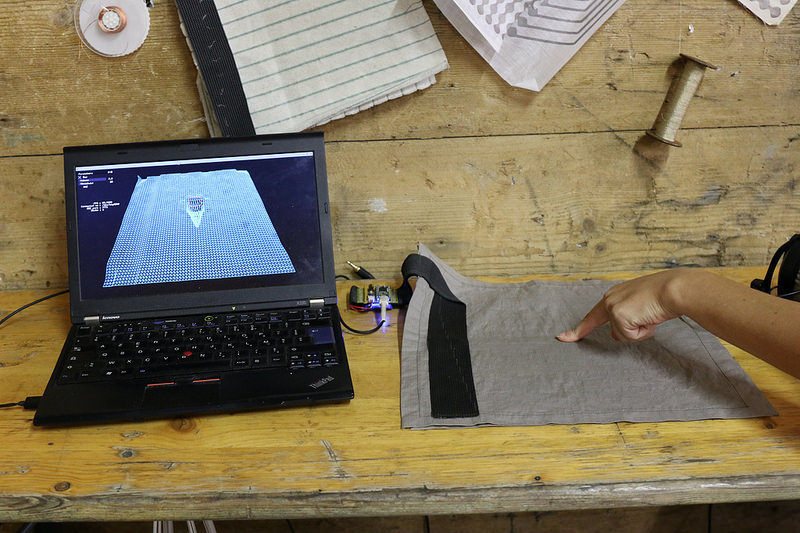
\includegraphics[width=\columnwidth]{figures/touch} }
%   \mbox{ \raisebox{3px}{ Visualization of the Robot Skin being touched.} }
}

% Make sure hyperref comes last of your loaded packages, to give it a
% fighting chance of not being over-written, since its job is to
% redefine many LaTeX commands.
\definecolor{linkColor}{RGB}{6,125,233}
\hypersetup{%
  pdftitle={\plaintitle},
%  pdfauthor={\plainauthor},
  pdfauthor={\emptyauthor},
  pdfkeywords={\plainkeywords},
  bookmarksnumbered,
  pdfstartview={FitH},
  colorlinks,
  citecolor=black,
  filecolor=black,
  linkcolor=black,
  urlcolor=linkColor,
  breaklinks=true,
}

% \reversemarginpar%

\begin{document}

\maketitle

% Uncomment to disable hyphenation (not recommended)
% https://twitter.com/anjirokhan/status/546046683331973120
\RaggedRight{}

% Do not change the page size or page settings.
\begin{abstract}
  UPDATED---\today. This sample paper describes the formatting
  requirements for SIGCHI Extended Abstract Format, and this sample
  file offers recommendations on writing for the worldwide SIGCHI
  readership. Please review this document even if you have submitted
  to SIGCHI conferences before, as some format details have changed
  relative to previous years. Abstracts should be about 150
  words. Required.
\end{abstract}

\keywords{\plainkeywords}

\category{H.5.m}{Information interfaces and presentation (e.g.,
  HCI)}{Miscellaneous}\category{See}{\url{http://acm.org/about/class/1998/}}{for
  full list of ACM classifiers. This section is required.}


\section{Introduction}


\subsection{What was done?}
This paper presents a soft, malleable, canvas, musical controller/instrument


\subsection{What is the (artistic) problem, or previously unfulfilled desire, that is addressed in this work?}
Current wearables are focused on visual aesthetics or functions, they do not address other dimensions of experience (touch, sound, smell etc.)
Current music devices are hard and rigid, with new materials emerging, we now have a desire for soft, malleable input.


\subsection{Why is this relevant? Why should the reader care?}
With technology becoming ubiquitous, it is shaping our bodies, our culture, our lives more and more. We need to design technologies for pleasure and expression rather than for productivity, if we in the future wish to lead pleasure full lives, rather than becoming productivity machines.


\subsection{What are other ways of solving your problem, addressing the unfulfilled desire? What did you not do and why? What did others do?}


This could just be half a paragraph or a sentence.
Here we can speak of the restricted scale of the sensor, originally the idea was to make a much larger interactive area to give a gesture dimension to musical interpretation.
We can also talk about the idea of designing a material as easy to work with as a traditional textile.


\subsection{How does what you did address the problem, the unfulfilled desire?}
This should compliment paragraph 2


\subsection{What is your contribution}
This can be a list or a sentence. You should state as clearly as possible what you are contributing to the conference/to the world. You have a two-part contribution:
- A soft instrument for artistic expression
- A method of creating this instrument
Related Work
Should be three or four paragraphs, I think


\subsection{Conceptually related work}
Hedonic/Soft/Wearable/Whatever you want to associate yourself with
http://dev-blog.mimugloves.com/


\subsection{Technologically related work}
https://atap.google.com/jacquard/


\subsection{Soft input devices / Material Sensors}
Kobakant stuff


\subsection{Related musical input devices/instruments}
There are several two-dimensional keyboard projects, this type of keyboard is referred to as 'harmonic keyboard', here are a few references: \cite{lambdoma}, \cite{seaboard}, \cite{linnstrument}, \cite{omnichord}.
The Omnichord is an instrument which offers a musical games that we want to adapt to the textile...


\section{Motivation / Discussion}

This is probably the hardest section, and should probably be written by Maurin. Why does he do what he does?


\subsection{Why did you build it? (what were the desires that needed to be fulfilled?)}
This textile sensor is the result of a reflection on the composition and the interpretation of electronic music. Result of a meeting between the world of weaving and electronics, I decided to develop this interface in textile in order to give a sensitive and intuitive dimension to controllers used to play electronic music.
Beyond the musical application, this textile sensor is a kind of artificial skin which give the "sense of touch" to objects. This technology may be used in a multitude of application fields such as connected objects, home automation, toys for children, wearable computing, etc.


\subsection{What is the history of this device?}
Elaborated in 2005 during my studies at the National School of Industrial Design (ENSCI - Paris), the first version of this textile interface only allowed to locate a single point of contact on the textile surface. In 2007 the project was oriented towards the development of a capacitive solution [using mixed digital/analog SoC - FPGA/FPAA] allowing to augment the sensitive faculties of the sensor, unfortunately undertaken developments have led us to abandon this too complex orientation [noise processing being a serious problem in wearable]. In 2014, in the Schmiede residence in Hallein (Austria), the project to found a new impetus [momentum?] through the development of a new piezoreistif textile based sensor. Today the development prospects multiply and the sensor adopts more and more the textile and digital qualities.


\subsection{What else did you try?}
This development is the result of a multitude of experiments in the field of electronic textiles. To develop each of the components of the sensor, many techniques had to be explored such as sewing, knitting, weaving, printing, etc. Several experiences were also made to pair this device to feedback solutions such as the video projection, lights in DMX control.


\subsection{How does this instrument satisfy what you wanted to do?}
In its current version, this interface offers a real solution for the composition and interpretation of electronic music. Robust, reactive and precise, it allows to trigger and control sounds...


\section{Implementation}

This is simply the technical implementation, probably Maurin and Cedric should write this, should be clear enough for non-experts to understand. If the motivation section is strong, this section can be skimmed over. I would try and not make this paper about the tech, but rather about Maurins vision and work.


\section{Presentation}

This section you write for the curator. Here you explain why the exhibit will be super cool if they pick you, and why they miss out on an amazing opportunity if they do not. You can edit/remove this if it gets accepted.


\subsection{How will visitors experience this piece of art?}
A performance? A demo? Maybe they can use it? Can anyone touch it? Will there be one or many?
It will be possible to play with a small models and a large version, the idea is also to present several textile experimentations to properly see the research project as a whole.


\subsection{Why does TEI want this}
It will be fun, people can walk up and use it. Because there are many devices, people can make music together, it will facilitate discussion, it will demonstrate all the themes of the topic:
- new materialities and morphologies
- material as interface, instrument
- material as expressive interactions
- human perception and materiality
- bio-hybrid systems and interactions
- materials on body


\section{Limitations and Future Work}

What does not work well yet?
What are opportunities for research based upon the things you have not managed to do?
What are opportunities for art, based on things you envision but did not do?
Conclusion
Summary of your submission document
Repeat your contribution in full
Repeat in two sentences why the curators should select your work

\balance{}

\bibliographystyle{SIGCHI-Reference-Format}
\bibliography{tei17}

\end{document}

%%% Local Variables:
%%% mode: latex
%%% TeX-master: t
%%% End:
